%! Author = itgramic
%! Date = 05.12.23

% Preamble
\subsubsection{Skalierung}
Datenbanken müssen skalierbar sein.
Dabei wird unterschieden zwischen einer vertikalen Skalierung (scale-up) und horizontaler Skalierung (scale-out).
Bei der vertikalen Skalierung werden den DB-Servern mehr CPU-Cores und Memory sowie zum Teil Storage hinzugefügt, wobei der Storage in jedem Fall wachsen wird.
Beim horizontalen Skalieren werden weitere DB-Nodes in den Cluster eingehängt\cite{IZSGZLVT}:
\begin{figure}[H]
    \centering
    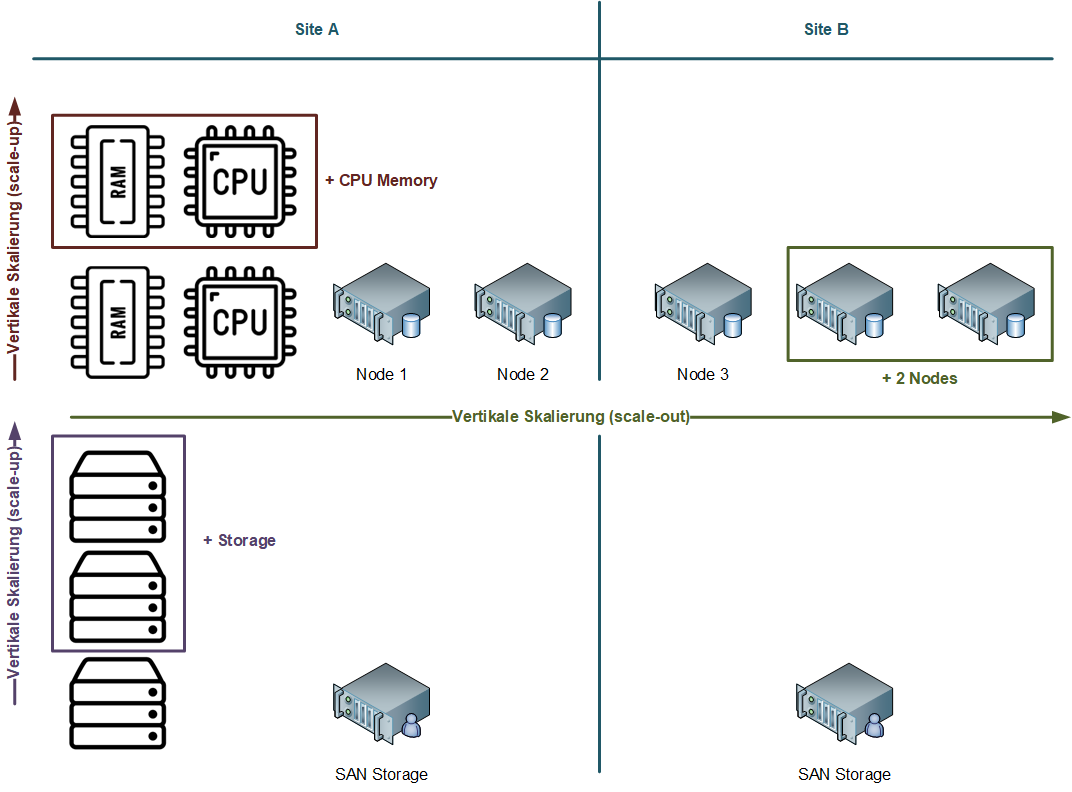
\includegraphics[width=1\linewidth]{source/implementation/evaluation/Skalierung}
    \caption{Datenbankskalierung}
    \label{fig:Datenbankskalierung}
\end{figure}